% !TEX root = ../main.tex
\chapter{Experiments}
\label{chapter:Experiments}

The current section describes the experiments which were conducted to assess the success of the implemented optimizations.
The chapter also compares the two sampling planners across three tracks and contrasts their behavior, raceline adherence, and lap-time performance.
The experiments were all conducted on one desktop workstation with an AMD Ryzen 9 5950X 16-Core Processor with SMT, 64 GB of DDR4 RAM, and an NVIDIA GeForce RTX 3090 GPU with 24GB of GDDR6X VRAM.

\section{Setup}
\label{section:Setup}

Before covering the contents of the experiments, it is equally important to first discuss how the DiffPlan and DiffSpatialPlan stacks interfaces with the simulator and the RoborRacer vehicle.
In terms of hardware and software compatibility, ROS2 was essential for running both environments for the real-life RoboRacer vehicle and the simulator.
ROS2 uses the Data Distribution Service (DDS) middleware for typed publish/subscribe communication between independent processes called nodes.
Each node exchanges messages on named topics, which allows the same planner executable to run in simulation or on the physical vehicle by swapping only the upstream and downstream nodes.

The differentiable planner is deployed as a ROS2 node.
It subscribes to the vehicle's pose topic and publishes drive commands on $\texttt{/drive}$.
All experiments use ground-truth ego localization rather than the differentiable DiffLoc module.
In simulation, pose is obtained from simulator odometry; on the physical vehicle, pose is provided by an OptiTrack motion-capture system through the $\texttt{vrpn\_mocap}$ package.
This configuration isolates planner performance from perception errors and benchmarks the planning and control stack in a controlled setting \cite{swadiryus_DifferentiableMotionPlanning_2025, koch_DifferentiableInterpretablePath_2025}.
The prediction module is also disabled in all runs.
No static obstacles or opponent vehicles are placed on the track, so experiments focus on solo lap-time optimization, raceline tracking, and wall avoidance \cite{koch_DifferentiableInterpretablePath_2025, swadiryus_DifferentiableMotionPlanning_2025}.

\begin{figure}[htbp]
    \centering
    \begin{subfigure}{\textwidth}
        \centering
        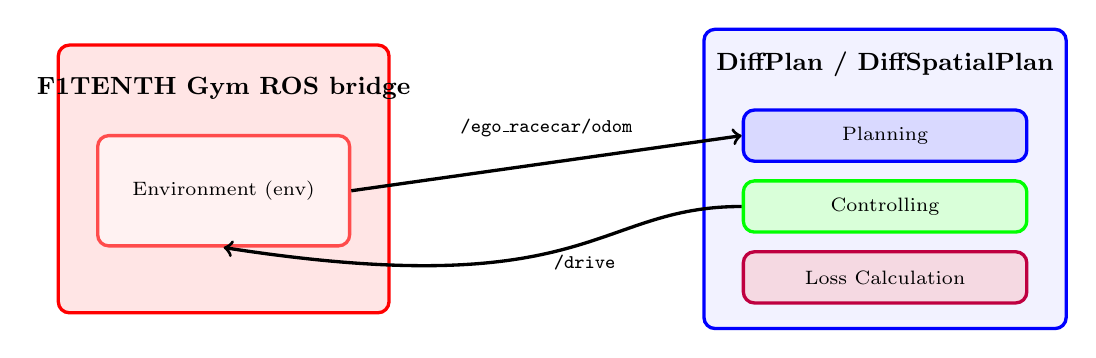
\begin{tikzpicture}[
            comp/.style={rectangle, draw, very thick, rounded corners, align=center, font=\small},
            inner/.style={rectangle, draw, very thick, rounded corners, align=center, font=\scriptsize},
            topic/.style={font=\scriptsize},
        ]
            % F1TENTH Gym ROS bridge (simulator)
            \node[comp, draw=red, fill=red!10, minimum width=4.2cm, minimum height=3.4cm] (gym) at (-4.2, 0) {};
            \node[font=\small\bfseries] at (-4.2, 1.15) {F1TENTH Gym ROS bridge};
            \node[inner, draw=red!70, fill=red!5, minimum width=3.2cm, minimum height=1.4cm] (env) at (-4.2, -0.15) {Environment (env)};

            % DiffPlan node
            \node[comp, draw=blue, fill=blue!5, minimum width=4.6cm, minimum height=3.8cm] (diffplan) at (4.2, 0) {};
            \node[font=\small\bfseries] at (4.2, 1.45) {DiffPlan / DiffSpatialPlan};
            \node[inner, draw=blue, fill=blue!15, minimum width=3.6cm, minimum height=0.65cm] (plan) at (4.2, 0.55) {Planning};
            \node[inner, draw=green, fill=green!15, minimum width=3.6cm, minimum height=0.65cm] (ctrl) at (4.2, -0.35) {Controlling};
            \node[inner, draw=purple, fill=purple!15, minimum width=3.6cm, minimum height=0.65cm] (loss) at (4.2, -1.25) {Loss Calculation};

            % Simulator data flow
            \draw[->, very thick] (env.east) -- node[topic, above=2mm] {$\texttt{/ego\_racecar/odom}$} (plan.west);
            \draw[->, very thick] (ctrl.west) .. controls (0.5, -0.35) and (0.5, -1.6) .. node[topic, below=0.5, pos=0.45] {$\texttt{/drive}$} (env.south);
        \end{tikzpicture}
        \caption{Simulation setup.}
        \label{fig:exp_setup_sim}
    \end{subfigure}

    \vspace{1.2em}

    \begin{subfigure}{\textwidth}
        \centering
        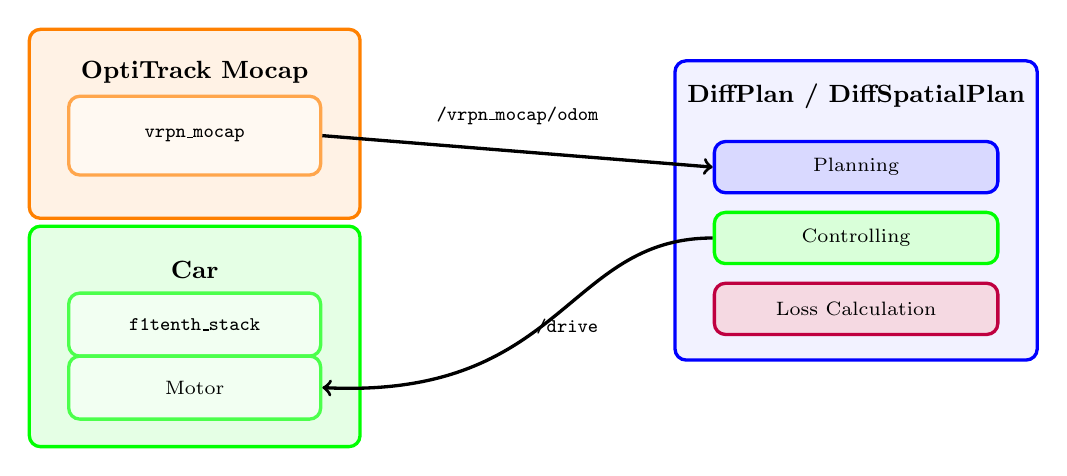
\begin{tikzpicture}[
            comp/.style={rectangle, draw, very thick, rounded corners, align=center, font=\small},
            inner/.style={rectangle, draw, very thick, rounded corners, align=center, font=\scriptsize},
            topic/.style={font=\scriptsize},
        ]
            % Motion capture system
            \node[comp, draw=orange, fill=orange!10, minimum width=4.2cm, minimum height=2.4cm] (mocap) at (-4.2, 1.1) {};
            \node[font=\small\bfseries] at (-4.2, 1.75) {OptiTrack Mocap};
            \node[inner, draw=orange!70, fill=orange!5, minimum width=3.2cm, minimum height=1.0cm] (vrpn) at (-4.2, 0.95) {$\texttt{vrpn\_mocap}$};

            % RoboRacer vehicle
            \node[comp, draw=green, fill=green!10, minimum width=4.2cm, minimum height=2.8cm] (car) at (-4.2, -1.6) {};
            \node[font=\small\bfseries] at (-4.2, -0.75) {Car};
            \node[inner, draw=green!70, fill=green!5, minimum width=3.2cm, minimum height=0.8cm] (stack) at (-4.2, -1.45) {$\texttt{f1tenth\_stack}$};
            \node[inner, draw=green!70, fill=green!5, minimum width=3.2cm, minimum height=0.8cm] (motor) at (-4.2, -2.25) {Motor};

            % DiffPlan / DiffSpatialPlan node
            \node[comp, draw=blue, fill=blue!5, minimum width=4.6cm, minimum height=3.8cm] (diffplan) at (4.2, 0) {};
            \node[font=\small\bfseries] at (4.2, 1.45) {DiffPlan / DiffSpatialPlan};
            \node[inner, draw=blue, fill=blue!15, minimum width=3.6cm, minimum height=0.65cm] (plan) at (4.2, 0.55) {Planning};
            \node[inner, draw=green, fill=green!15, minimum width=3.6cm, minimum height=0.65cm] (ctrl) at (4.2, -0.35) {Controlling};
            \node[inner, draw=purple, fill=purple!15, minimum width=3.6cm, minimum height=0.65cm] (loss) at (4.2, -1.25) {Loss Calculation};

            % Real-world data flow
            \draw[->, very thick] (vrpn.east) -- node[topic, above=2mm] {$\texttt{/vrpn\_mocap/odom}$} (plan.west);
            \draw[->, very thick] (ctrl.west) .. controls (0.5, -0.35) and (0.5, -2.4) .. node[topic, below=1, pos=0.45] {$\texttt{/drive}$} (motor.east);
        \end{tikzpicture}
        \caption{Physical RoboRacer setup.}
        \label{fig:exp_setup_real}
    \end{subfigure}
    \caption{Experimental control loops in simulation and on the physical RoboRacer vehicle.
    In both setups, ground-truth pose feeds the planner stack, which returns $\texttt{/drive}$ commands to the plant.
    DiffLoc and prediction remain disabled in all benchmark runs.}
    \label{fig:exp_setup}
\end{figure}

\subsection{Simulation Setup}

The simulator is based on O'Kelly et al.\ \cite{okelly_F1TENTHOpensourceEvaluation_2019} F1TENTH Gym, containerized and adapted to ROS2 through the $\texttt{f1tenth\_gym\_ros}$ bridge.
Three track maps are used in the planner comparison: FTM Oval, Austria, and Yas Marina.
The ROS2 simulator node initializes the selected track map, spawns the ego vehicle, and simulates the vehicle dynamics at each control timestep.
It publishes odometry on $\texttt{/ego\_racecar/odom}$ and subscribes to throttle and steering commands on $\texttt{/drive}$.
Although the simulator exposes LiDAR and other perception topics, these streams are not consumed because all experiments rely on ground-truth pose.
Contrarily, The workstation desktop which runs the planner stacks subscribes to the odometry topic $\texttt{/ego\_racecar/odom}$ and publishes the $\texttt{/drive}$ topic for the simulator environment.

\subsection{Real Life Setup}

The setup includes three pieces of hardware collaborating over ROS2.
The RoboRacer vehicle runs the $\texttt{f1tenth\_stack}$ package, the onboard ROS2 software stack that exposes sensor drivers and actuation $\texttt{/drive}$ commands to motor and steering outputs \cite{okelly_F1TENTHOpensourceEvaluation_2019, betz_TUMAutonomousMotorsport_2023}.
Eight motion-capture cameras surrounds the real-life circuit and keep track of three motion-capture markers across the RoboRacer vehicle's frame obtaining the position and heading of the vehicle.
The pose and heading data are streamed over ROS2 through the $\texttt{vrpn\_mocap}$ package to the workstation desktop which runs the DiffPlan or DiffSpatialPlan stacks.
The planner subscribes to the pose topic $\texttt{/vrpn\_mocap/odom}$ and publishes $\texttt{/drive}$ commands to the car to actuate its motors for acceleration and steering.
Figure \ref{fig:exp_setup} illustrates the communication layout in ROS2 between different hardware nodes with Figure \ref{fig:exp_setup_sim} describing the simulation setup and Figure \ref{fig:exp_setup_real} describing the real-life setup.


\section{Optimization}
\label{section:Optimization}

This section describes the experiments that were performed to measure the degree of optimization that was accomplished.
As stated in Chapter \ref{chapter:optimizations}, these experiments follow the vectorization of two inefficient for loop blocks that slowed down the simulation pipeline.
The original longitudinal sampling and wall collision loss calculation algorithms were vectorized to take advantage of SIMD (Single Instruction, Multiple Data) parallelism \cite{flynn_ComputerOrganizationsTheir_1972}.
By applying the same operation to multiple data elements in parallel, SIMD reduces per-iteration loop overhead and improves memory access patterns across contiguous tensor blocks \cite{paszke_PyTorchImperativeStyle_2019}.
Two major metrics will be looked at: first the full runtime of the algorithm will be assessed, and second the planning runtime will be measured as the number of sampled trajectories increases.
The initial subsection \ref{subsection:Runtime} will focus on measuring runtime of the four algorithms presented previously and compare them.
Additionally, the scalability of the four algorithms will be assessed as the number of sampled trajectories increases.

\subsection{Runtime}
\label{subsection:Runtime}

The aim of this experiment is to compare the runtimes of the original, vectorized, and GPU-offloaded versions of the temporal sampling planner together with the spatial sampling planner DiffSpatialPlan.
This is done by taking a profile trace of each algorithm using the PyTorch profiler.
The profiler records all traversed functions that it encounters and the length of time each function took; the trace is saved as a JSON file for offline analysis.
Each algorithm was profiled consistently at the same start and end points so as not to contaminate any comparisons.
The experiment was run five times to prevent any outlier data from dominating the measurement, and the runs were averaged to obtain a final time for each section.
This experiment is track agnostic as the overall runtime is not dependent on what track is being traversed.

\subsection{Scaling}
\label{subsection:Scaling}

The purpose of the scaling experiment is to ascertain information about the runtime behavior of the respective planning algorithms as the number of sampled trajectories $n$ grows.
It indicates how the algorithm's computational complexity grows relative to the problem size.
The PyTorch profiler is again used for these measurements, saved as a JSON file.
For each value of $n$, the measurement was repeated five times and averaged to reduce the influence of outliers, following the same approach as the runtime experiment in Subsection~\ref{subsection:Runtime}.

\section{Local Sampling Planner}
\label{section:DiffPlanAndDiffSpatialPlan}

This section covers the experiments performed on the simulator and on the physical vehicle pertaining to the differences between the temporal sampler DiffPlan and the spatial sampler DiffSpatialPlan.
The overall software and hardware architecture for simulation and real-world deployment is described in Section~\ref{section:Setup} and Figure~\ref{fig:exp_setup}.
The experiments utilize simulation and real runs to draw conclusions about the individual runs as well as a combined simulation-versus-real comparison.
On the FTM Oval track, identical conditions were used for both simulation and real-world runs to draw insights into the sim-to-real gap that must be overcome.
Two other tracks are only available in simulation.
All tracks were used to test how each algorithm showcases local planning ability, path tracking toward the global goal, and lap-time performance.

Henceforth, all tracks both in simulation and physical, the vehicle was placed initially offset from the raceline with the following initial values for the cost function weights,
\begin{equation*}
    \theta_{\text{curv}} = 0.5, \ \theta_{\text{vel}} = 7.5, \ \theta_{\text{rl}} = 0.5, \ \text{else} \ \theta = 1.0,
\end{equation*}
and the following loss function objective was described:
\begin{equation}
    \mathcal{L}_{\text{total}} = \alpha_{\text{prog}}\,\mathcal{L}_{\text{prog}} + \alpha_{\text{coll}}\,\mathcal{L}_{\text{coll}} + \alpha_{\text{rl}}\,\mathcal{L}_{\text{rl}},
    \label{eq:VecDiffPlanLoss}
\end{equation}
where $\alpha_{\text{prog}} = 1.0$, $\alpha_{\text{coll}} = 1.0$, and $\alpha_{\text{rl}} = 5.0$, while the individual loss functions can be found in Eq \ref{eq:DiffPlanProgLoss}, \ref{eq:DiffPlanCollLoss}, and \ref{eq:DiffPlanRlLoss} respectively.
This configuration was inspired by Swadiryus \cite{swadiryus_DifferentiableMotionPlanning_2025}, who initializes cost function weights $\theta$ with strong emphasis on velocity deviation and comparatively low weight on raceline adherence.
The trainable weights are updated at each control step using the Adam optimizer \cite{kingma_AdamMethodStochastic_2015} with learning rate $10^{-3}$, applying the gradients of $\mathcal{L}_{\text{total}}$ with respect to the planner cost parameters.
With the objective in Equation \ref{eq:VecDiffPlanLoss}, the experiments test whether the planner can learn a more effective configuration of $\theta$ over training.

The following metrics will be gathered and evaluated for each track and for both planners:
\begin{itemize}
    \setlength\itemsep{2pt}
    \item Vehicle trajectory per lap, plotting how the driven path evolves over training.
    \item Lateral deviation from the global raceline
    \item Lap time
    \item Per-lap values of the loss terms in Equation~\ref{eq:VecDiffPlanLoss}: progress loss $\mathcal{L}_{\text{prog}}$, collision proximity loss $\mathcal{L}_{\text{coll}}$, and raceline deviation loss $\mathcal{L}_{\text{rl}}$
\end{itemize}

\subsection{Simulation Runs}

All simulated tracks are scaled appropriately for the RoboRacer vehicles.
The tracks are encapsulated in simulation using three files: A png image of the track including boundaries, accompanying a yaml file which contains specific information pertaining to the track such as origin location and resolution, and finally a csv file which contains the full description of the raceline.
The global raceline contains a discretized description of the following metrics along with its associated unit: The longitudinal progress $s (m)$, cartesian positions $x (m), y (m)$, global heading $\psi (\text{rad})$, curvature of track $\kappa (\text{rad}/m)$, velocity $v_x (m/s)$, acceleration $a_x (m/s^2)$.
All three of the files are used in the simulation to help the vehicle reason about its current objective.

\subsubsection{FTM Oval}

% add image of the track with raceline
The FTM Oval track is a real track found at Chair of Autonomous Technology at the Technical University Munich which was specifically built for RoboRacer vehicles.
It features a small oval track that provides adequate feedback of the performance of autonomous RoboRacer vehicles.
This track was converted to the three files mentioned above to be used in simulation.
Fig \ref{fig:ftm-oval-track} shows the track layout as well as the initial starting position of the car.

\begin{figure}[htbp]
    \centering
    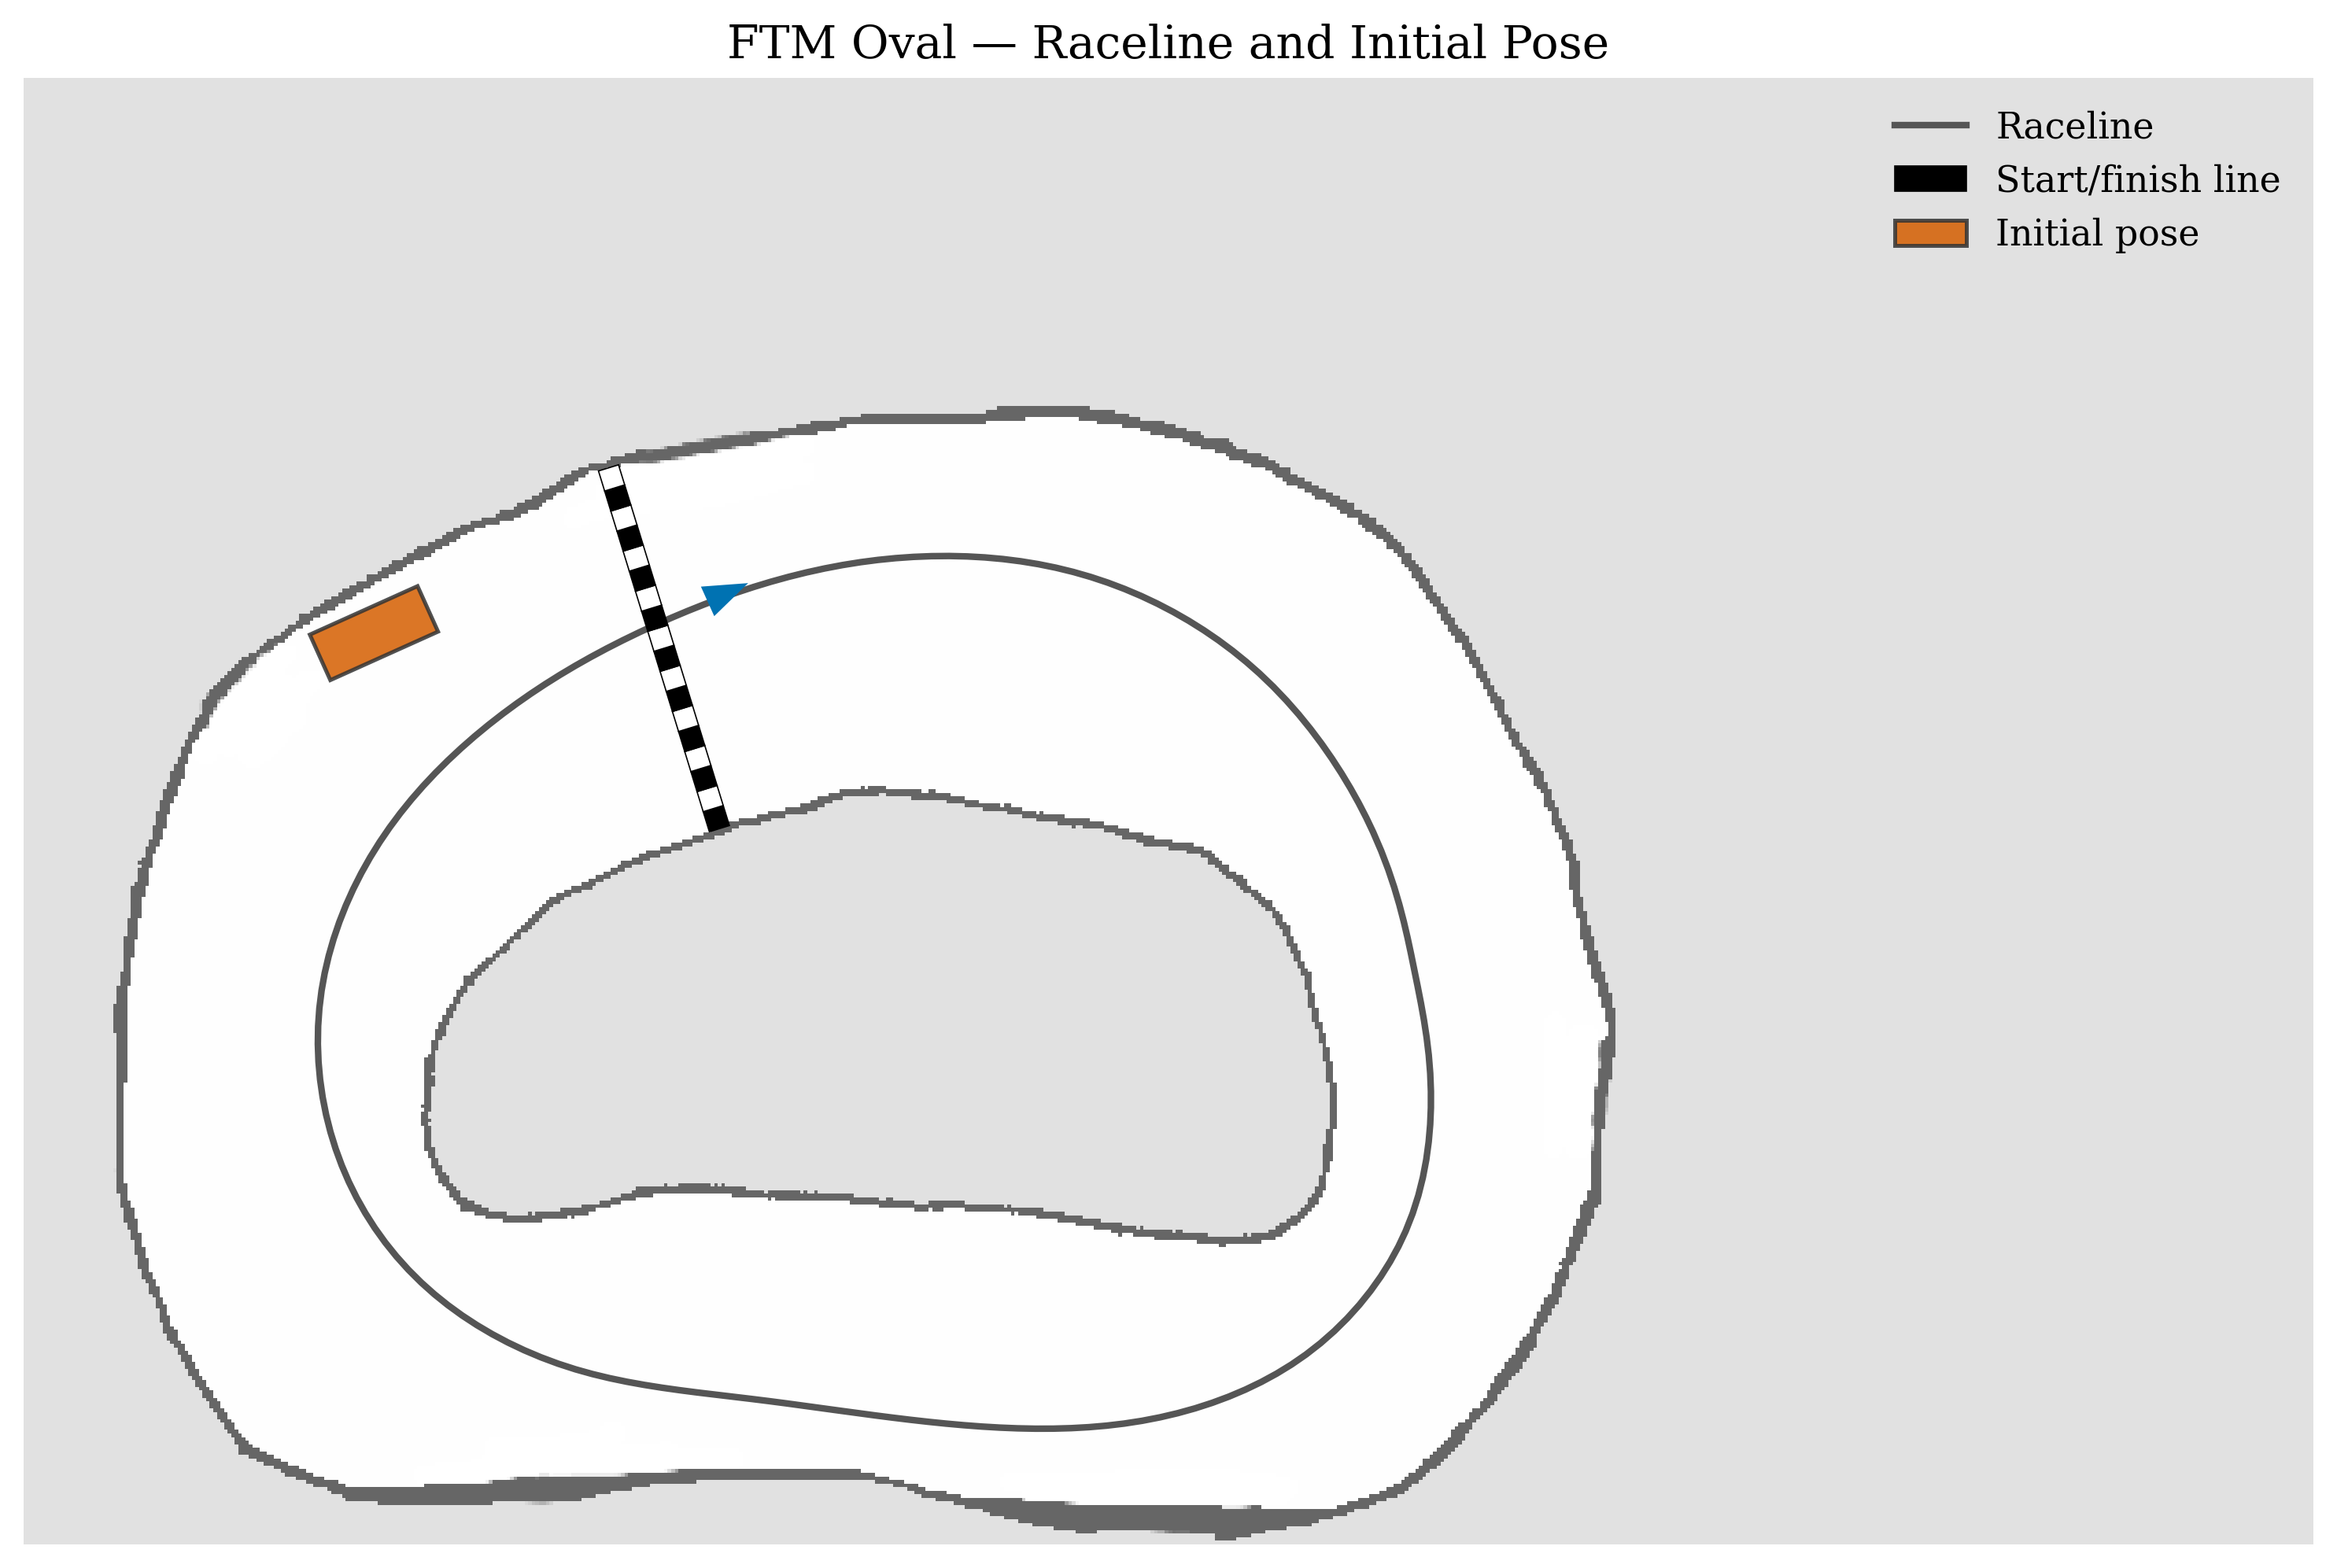
\includegraphics[width=0.7\linewidth]{images/ftm_oval_track.png}
    \caption{FTM Oval track and initial position of the vehicle (orange box)}
\label{fig:ftm-oval-track}
\end{figure}

\subsubsection{Yas Marina Track}

This track is modelled after the Yas Marina Formula 1 circuit in the Abu Dhabi Grand Prix but adapted to RoboRacer scale.
The circuit in Fig \ref{fig:yas-marina-track} features a portion of the complex cornering found in the full circuit with two $180^\circ$ hairpin turns and a series of corners that closely follow each other.
The combination of high speed driving and slow corners provide adequate conditions to test the capabilities of both planning algorithms.

\begin{figure}[htbp]
    \centering
    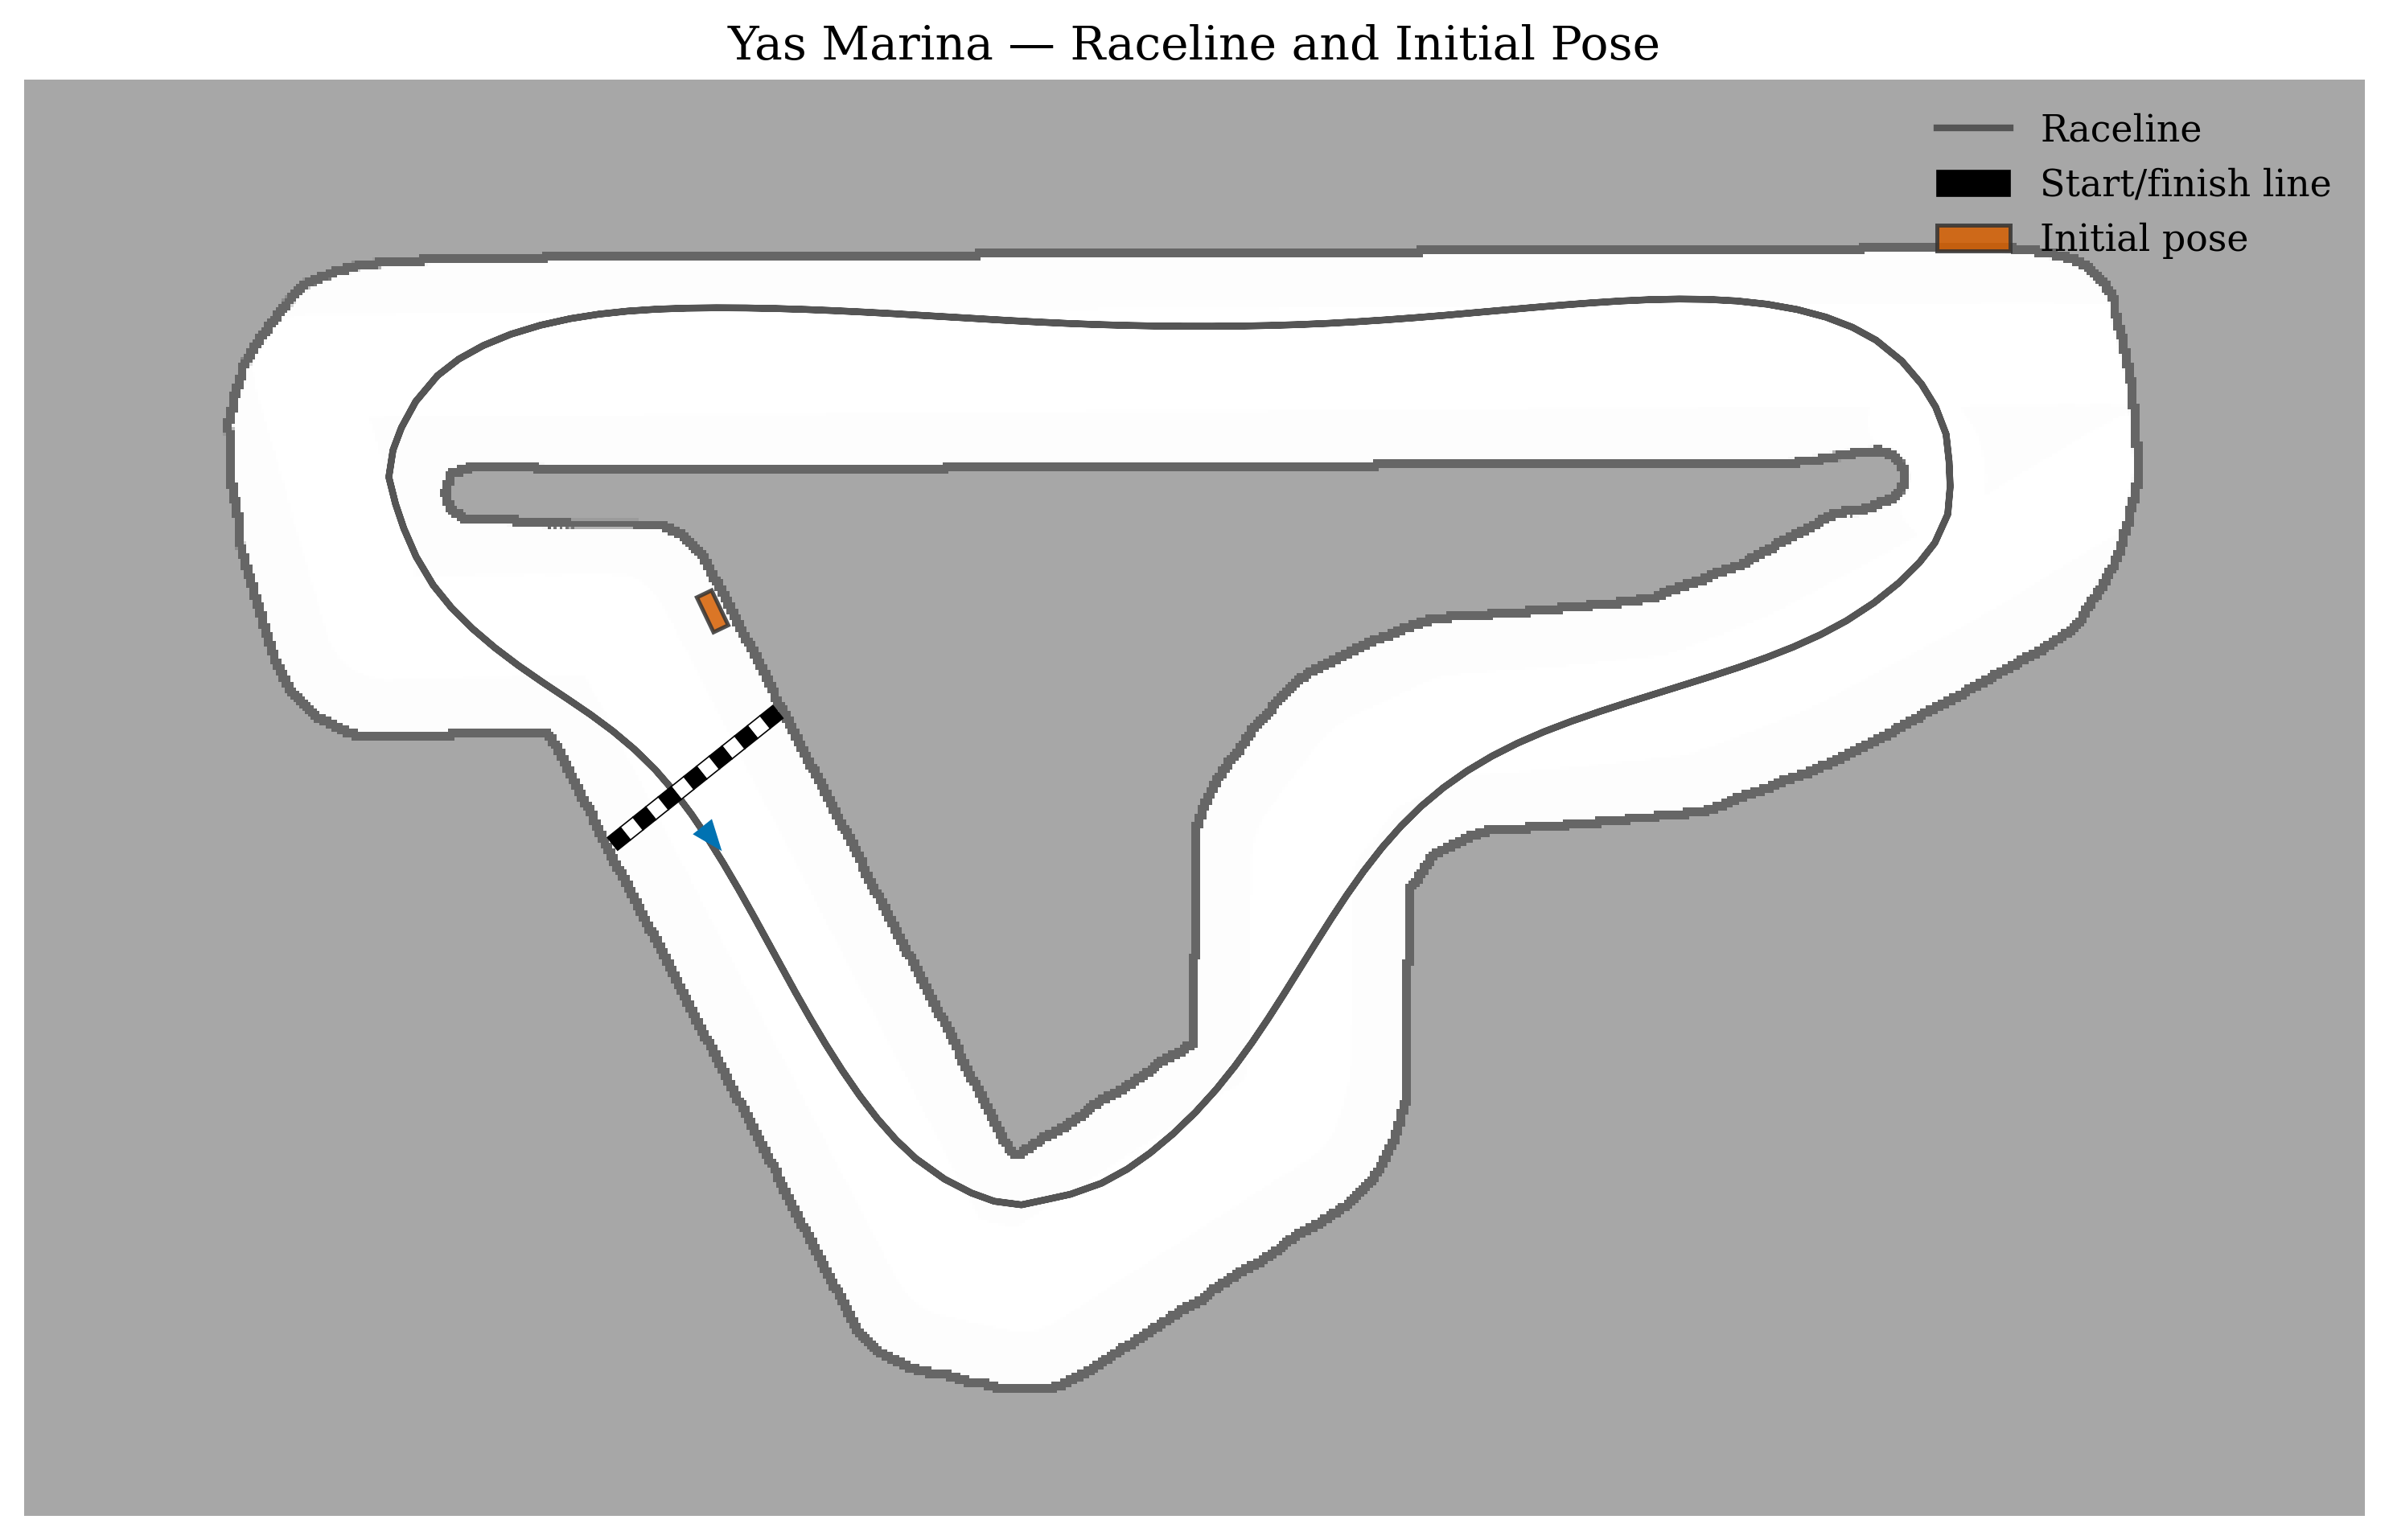
\includegraphics[width=0.7\linewidth]{images/yas_marina_track.png}
    \caption{Yas Marina track and initial position of the vehicle (orange box)}
\label{fig:yas-marina-track}
\end{figure}

% \newpage
\subsubsection{Austria Track}

Once again the track is a RoboRacer adaptation of the Red Bull Ring used in the Austrian Grand Prix in Formula 1 which can be seen in Fig \ref{fig:austria-track}.
The track features high speed racing line with high curvature corners and tight adherence to the track boundaries.
Benchmarking the driving stacks with balancing raceline adherence, maintaining high speed, and careful maneuvering to not crash into the barriers. 

\begin{figure}[htbp]
    \centering
    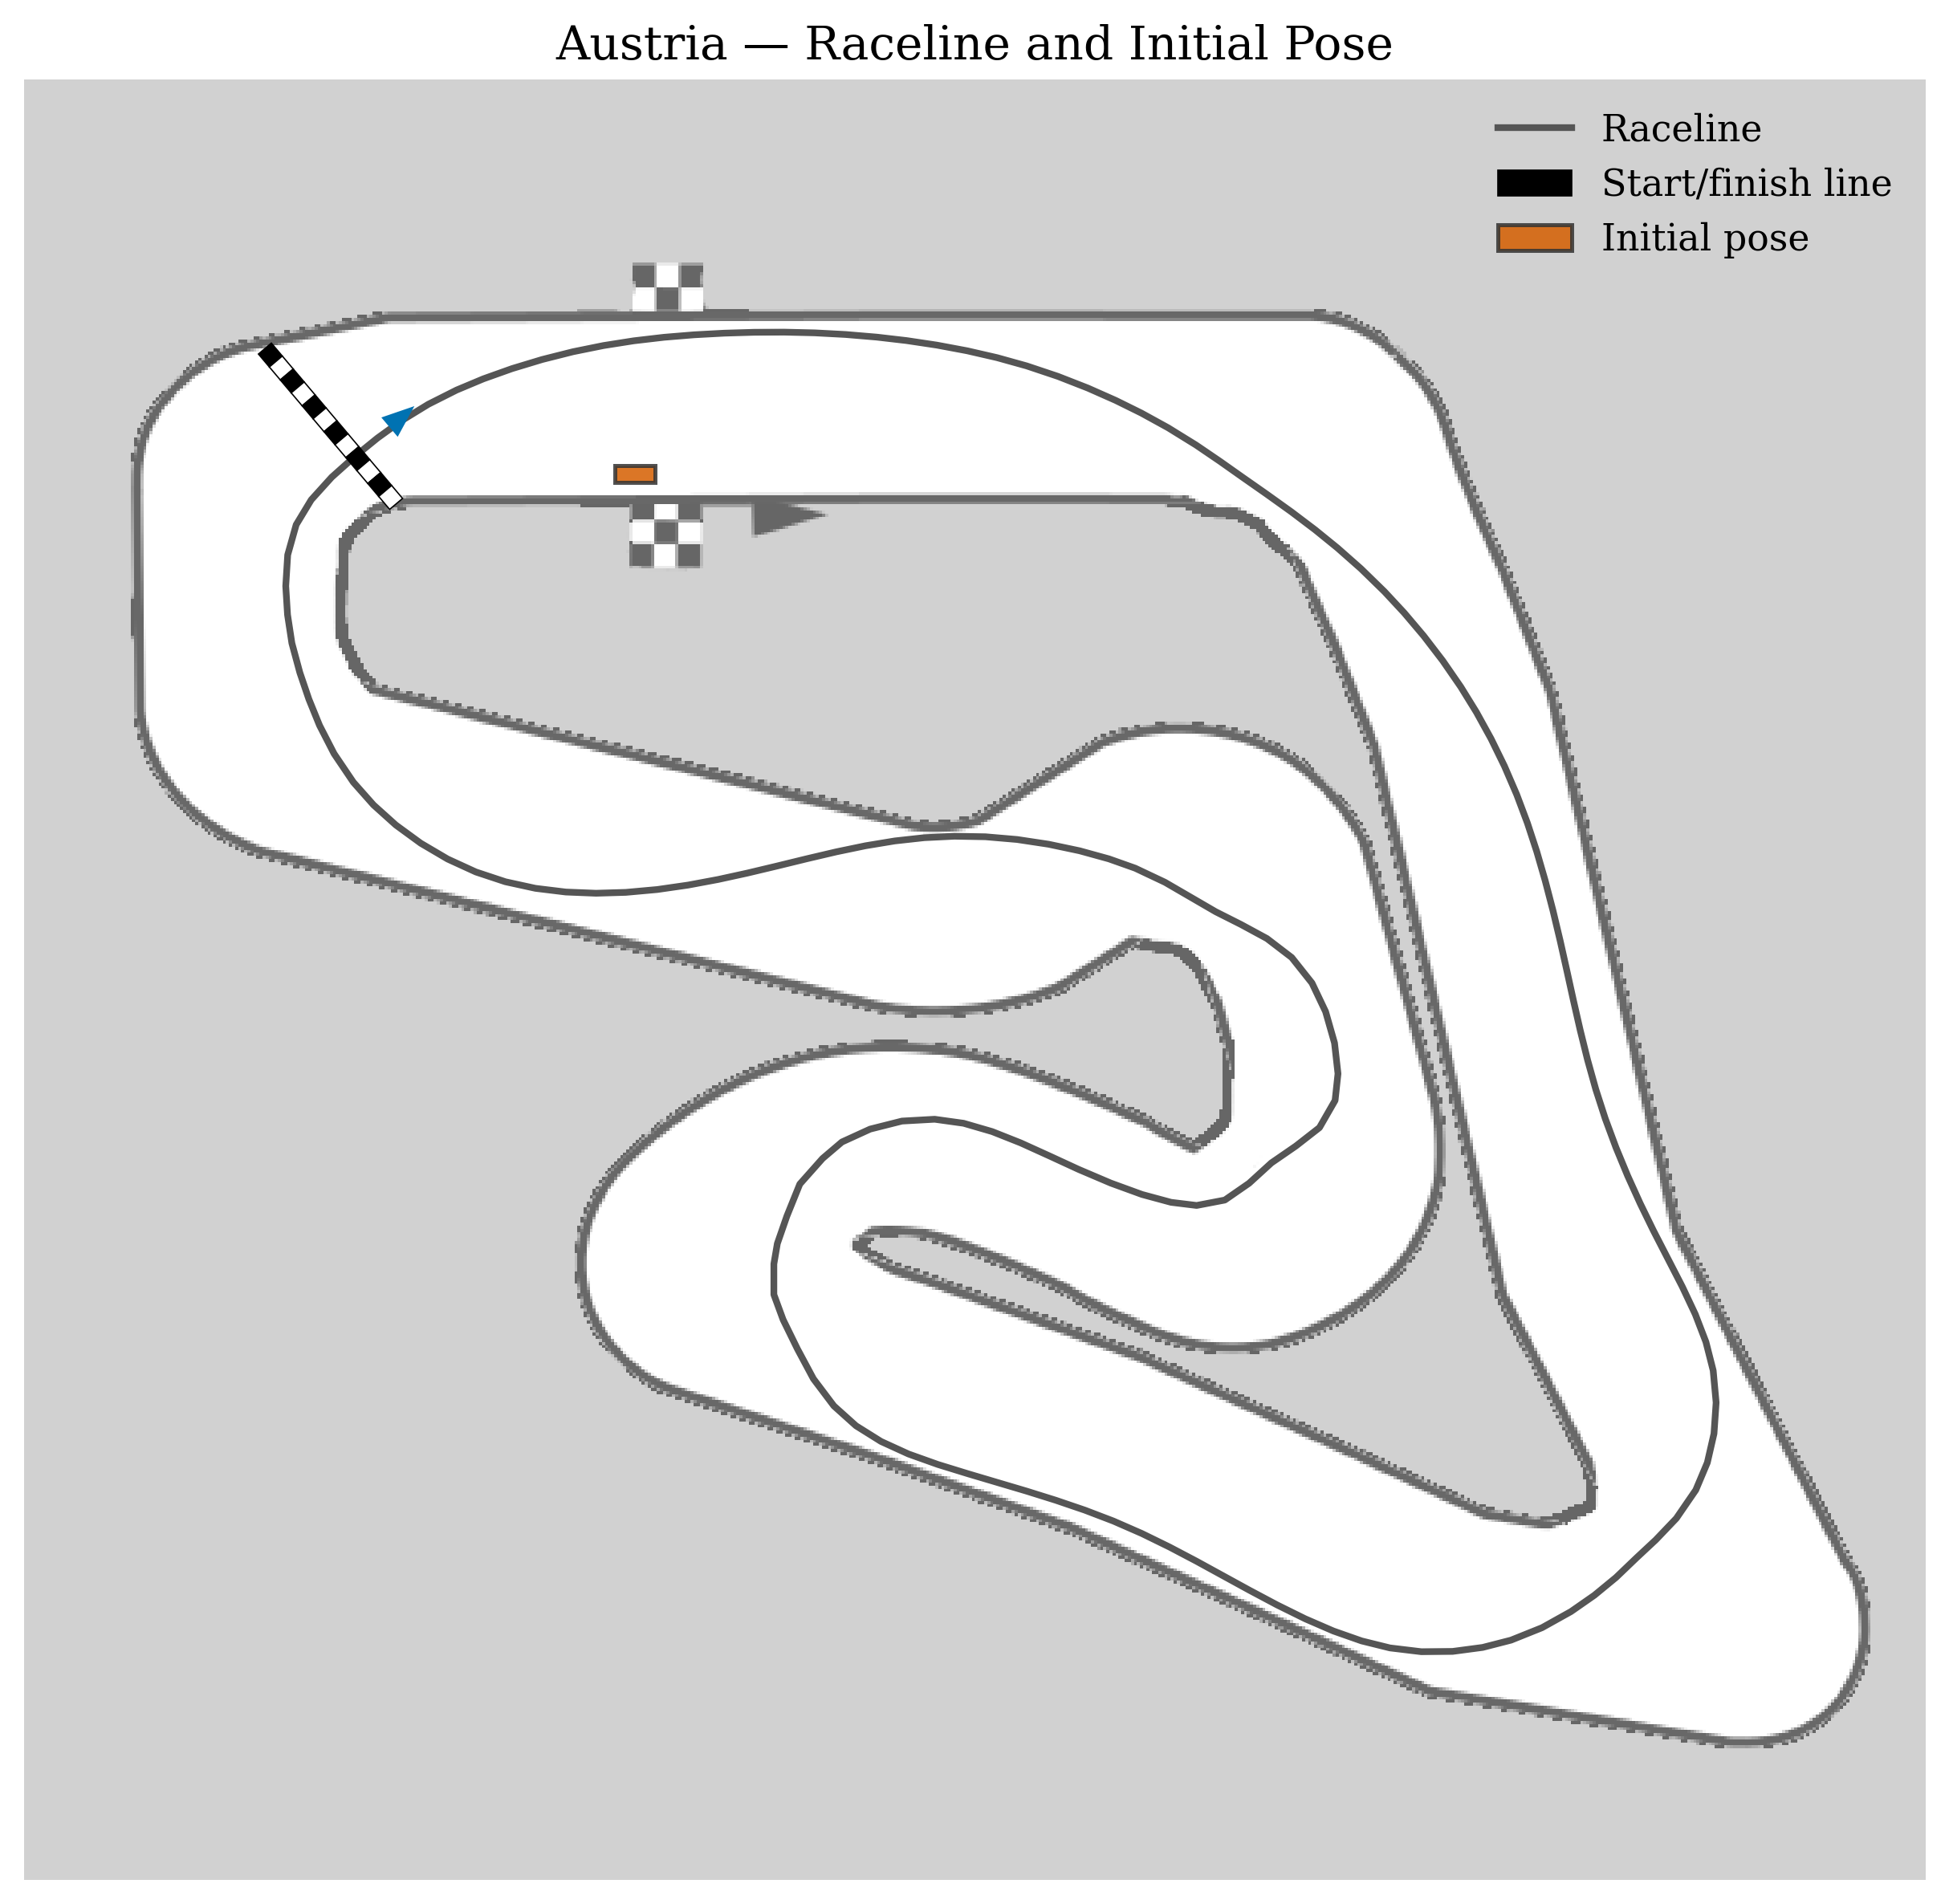
\includegraphics[width=0.7\linewidth]{images/austria_track.png}
    \caption{Austria track and initial position of the vehicle (orange box)}
\label{fig:austria-track}
\end{figure}

\subsection{Real Runs}

As the mentioned previously, the FTM Oval track was used to validate the physical deployment of two local motion planners.
The starting position of the car was marked on the physical track using colored tape to ensure consistency between runs.
